\documentclass[a4paper]{article}
\usepackage[utf8]{inputenc}
\usepackage[english]{babel}
\usepackage{amsmath} % per ambienti tipo cases
\usepackage{amssymb}
\usepackage{mathtools}
\usepackage{siunitx}
\usepackage{graphicx} % per includere figure
%\usepackage{subfigure}
\usepackage{booktabs} % per le tabelle
\usepackage{caption}
\usepackage{fancyhdr}
\usepackage{hyperref}
\usepackage[section]{placeins}
\usepackage{microtype}
\usepackage{caption}
\usepackage{subcaption}
\captionsetup[subfigure]{labelfont=rm}
\usepackage{verbatim} %multiline comments
\usepackage{wrapfig}
%\usepackage[backend=biber, style=numeric, safeinputenc, sorting=none]{biblatex}
%\addbibresource{source.bib}	% uncomment for bibliography



%opening
\title{}
\author{}

\pagestyle{fancy}
\lhead{Musical Acoustics}
\chead{H5}
\rhead{10743504, 10751919}
\newcommand{\Rarrow}{\mbox{\Large$\Rightarrow$}}

\begin{document}

\begin{titlepage}	
	\newcommand{\HRule}{\rule{\linewidth}{0.5mm}} % Defines a new command for horizontal lines, change thickness here
	
	\center % Centre everything on the page
	
	%------------------------------------------------
	%	Headings
	%------------------------------------------------
	
	
\includegraphics[width=.4\textwidth]{Logo_Politecnico_Milano.png}\\[0.4cm]
	\textsc{\LARGE}\\[0.3cm] % Main heading such as the name of your university/college
	
	\textsc{\large MSc. Music and Acoustic Engineering}\\[1cm] % Minor heading such as course title
	
	\textsc{\Large Musical Acoustics - A.Y. 2020/2021}\\[0.5cm] % Major heading such as course name
	
	%------------------------------------------------
	%	Title
	%------------------------------------------------
	
	\HRule\\[0.4cm]
	
	{\huge\bfseries H5 - Synthesis of the guitar sound }\\[0.4cm] % Title of your document
	
	\HRule\\[1.5cm]
	
	
	
	{\large\textit{Authors' IDs:}}\\
	10743504, 10751919, % Your name
	%\\ \textsc{Gruppo 11}
	
	%------------------------------------------------
	%	Date
	%------------------------------------------------
	
	\vfill\vfill\vfill % Position the date 3/4 down the remaining page
	
	{\large\today} % Date, change the \today to a set date if you want to be precise
	
	%------------------------------------------------
	%	Logo
	%------------------------------------------------
	
	\vfill\vfill
	%\includegraphics[width=0.2\textwidth]{Politecnico_di_Milano.eps}\\[1cm] % Include a department/university logo - this will require the graphicx package
	
	%----------------------------------------------------------------------------------------
	
	\vfill % Push the date up 1/4 of the remaining page
	
	
\end{titlepage}

\section{Bridge impedance}
The bridge impedance is computed as the ratio between the pressure on the top plate (the force applied to the top plate divided by the effective top plate area) and the volume velocity of the plate itself. The guitar body is modelled as a two-mass system, neglecting the back plate and the ribs, and each element is assumed to be lumped, a reasonable assumption considering that we are interested in the frequencies below 500 Hz. The elements in question are the top plate, the air cavity and the sound hole, and their impedances are:
\begin{align*}
	Z_p &= \mathrm{j}\omega M_p + R_p + \frac{1}{\mathrm{j}\omega C_p}, \quad &\text{where } M_p = \frac{m_p}{A_p^2}, ~ C_p = \frac{A_p^2}{K_p} \\
	Z_v &= \frac{1}{\mathrm{j}\omega C_v} + R_v, \quad &\text{where } C_v = \frac{V}{\rho c^2} \\
	Z_h &= \mathrm{j}\omega M_h + R_h \quad &\text{where } M_h = \frac{m_h}{A_h^2}.
\end{align*}

The system can be thought of as composed of two coupled oscillators: one is the top plate, while the other is the  cavity/sound hole resonator. The resulting equivalent circuit can be seen in Fig. \ref{fig:2mass}.


\begin{wrapfigure}{R}{0.4\linewidth}
	\centering
	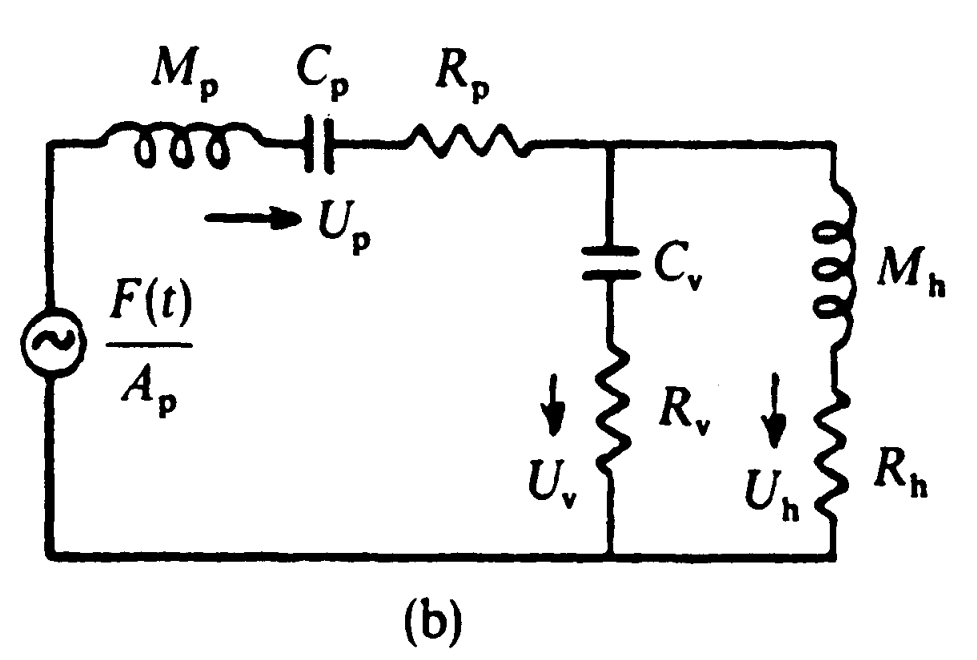
\includegraphics[width=\linewidth]{2mass.png}
	\caption{Two-mass model of the guitar body.}
	\label{fig:2mass}
\end{wrapfigure}

The input impedance of this circuit is the series of $Z_p$ with the parallel of $Z_v$ and $Z_h$
$$ Z = Z_p + \frac{Z_v Z_h}{Z_v + Z_h} .$$
The magnitude and phase of $Z$ as functions of the frequency are shown in Fig. \ref{fig:brimp}. The magnitude graph shows two points of resonance with one anti-resonance in between, as expected. The antiresonance corresponds to the Helmholtz resonance frequency $f_h$ of the cavity/sound hole subsystem (the $A_0$ mode of the cavity). The highest resonance occurs at the resonance frequency $f_p$ of the system without the sound hole. This tells us that the effects of the losses due to the resistances are very small, since these frequencies are computed for the conservative case.

\begin{figure}[h]
	\centering
	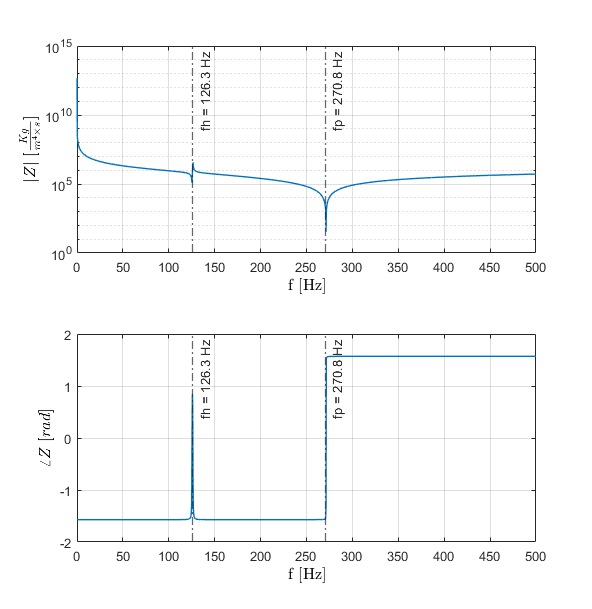
\includegraphics[width=0.75\linewidth]{bridge_impedance.png}
	\caption{Bridge impedance as a function of the frequency. The values of $f_h$ and $f_p$ are highlighted.}
	\label{fig:brimp}
\end{figure}


 \begin{table}[h]
 	\centering
 	$\begin{array}{lc}
 		\toprule
 		C_p & \SI{1.48e-9}{\newton\per\meter^5}\\
 		M_p & \SI{236.4}{\kilogram\per\meter\squared}\\
 		R_p & \SI{32.0}{\newton\second\per\meter^5}\\
 		\midrule
 		C_v & \SI{1.22e-7}{\newton\per\meter^5}\\
 		R_v & 0\\
 		\midrule
 		M_h & \SI{13.05}{\kilogram\per\meter\squared}\\
 		R_h & \SI{30.0}{\newton\second\per\meter^5}\\
 		\bottomrule
 	\end{array}$
	 \caption{Values of the compliances, inertances and resistances of the system.}
	\label{tab:vals}
 \end{table}


\section{Transfer function from the plucking point to the bridge}

\begin{figure}[h]
	\centering
	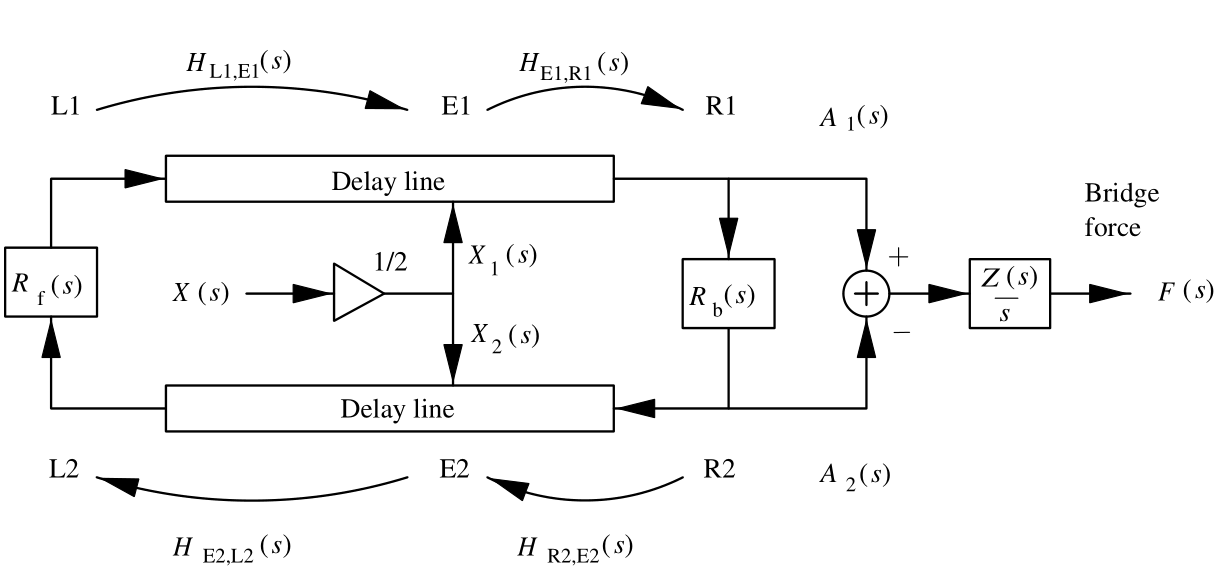
\includegraphics[width=0.7\linewidth]{synth.png}
	\caption{Model of the bidirectional waveguide model coupled with the bridge impedance $Z(s)$.}
	\label{fig:dwg}
\end{figure}

A guitar string can be modelled as two transmission lines in opposite directions with two reflection filters at the end points (see Fig. \ref{fig:dwg}), with the input being given at a certain fraction $\beta$ of the length. This model can be implemented easily with digital waveguides, as is done in most synthesis applications.  However, if the model is an LTI system, its components can be commuted to obtain a single-delay loop (SDL), resulting in an increase in efficiency, which is a desirable feature in real time synthesis\cite{kar98}. When we use acceleration as a wave variable, the transfer function of the system is:

\begin{align*}
	H_{EB}(s) = &\frac{1}{2}\biggl[ 1 + H_{E2R1}(s) \biggr] \frac{H_{E1R1}(s)}{1 - H_{loop}(s)} Z(s) \frac{1}{s} \biggl[ 1 - R_b(s) \biggr] = \\[5pt] =~ &H_E (s) H_{E1R1}(s) S(s) H_B(s) 
\end{align*}

Here $H_E(s)X(s)$ is the sum of the part of the input that is fed directly to one of the delay lines at E1 with the other half after it has travelled from the excitation point E2 to the nut, where it goes through the reflection filter, and back again along the first line to the excitation point E1. This lets us consider the excitation as if it were happening at a single point, with a lumped input filter. Fig. \ref{fig:he} shows our implementation of this filter, with a discrete delay that was computed as the product of the time delay with the sampling frequency and the losses being represented as a multiplying factor slightly less than 1.

The filter $H_{E1R1}(s)$ represents the transmission of the excitation signal from E1 to the bridge, and here it is modeled by the series of a delay and a loss factor (see Fig. \ref{fig:he1r1}).

We then have $S(s) = \frac{1}{1 - H_{loop}(s)}$, where $H_{loop}(s)$ is the transfer function of a single loop of the signal from the bridge to the nut and back to the bridge. This part is represented as a feedback loop, shown in Fig. \ref{fig:s}, and the feedback filter is the series of a loss factor, a delay (corresponding to twice the time necessary for the signal to travel the length of the string) and a lowpass. The lowpass was implemented with a 2-point moving average, like in the Karplus-Strong algorithm.

Finally, we have the bridge filter $H_B(s) = Z(s)\frac{1}{s} \left[ 1 - R_b(s) \right]$. This represents the load due to the bridge (and body) of the guitar and therefore we will use the impedance we obtained earlier as $Z(s)$. The reflection filter of the bridge can be considered roughly constant and equal to -1, thus the gain factor of 2. The integrator is needed because, as mentioned earlier, we are using the acceleration as the wave variable.

\begin{figure}[h]
	\centering
	\begin{subfigure}{0.47\linewidth}
		\centering
		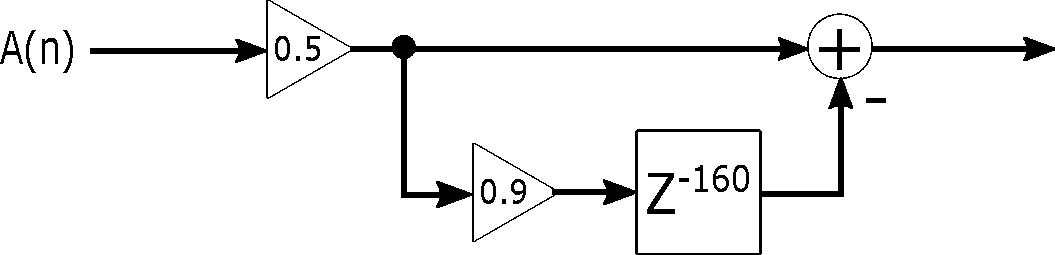
\includegraphics[width=0.9\linewidth]{H_E.pdf}
		\caption{}
		\label{fig:he}
	\end{subfigure}
	~
	\begin{subfigure}{0.47\linewidth}
		\centering
		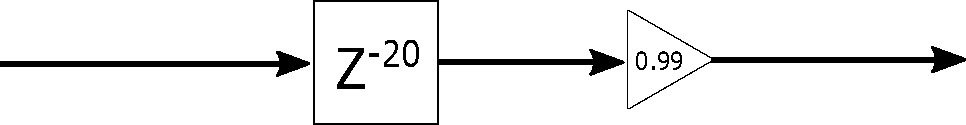
\includegraphics[width=0.9\linewidth]{H_E1R1.pdf}
		\caption{}
		\label{fig:he1r1}
	\end{subfigure}

	\begin{subfigure}{0.47\linewidth}
		\centering
		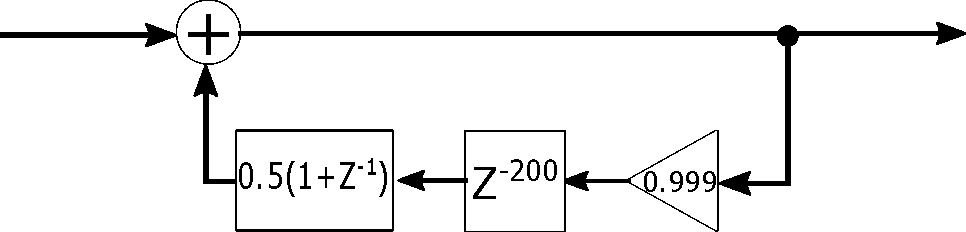
\includegraphics[width=0.9\linewidth]{S.pdf}
		\caption{}
		\label{fig:s}
	\end{subfigure}
	~
	\begin{subfigure}[b]{0.47\linewidth}
		\centering
		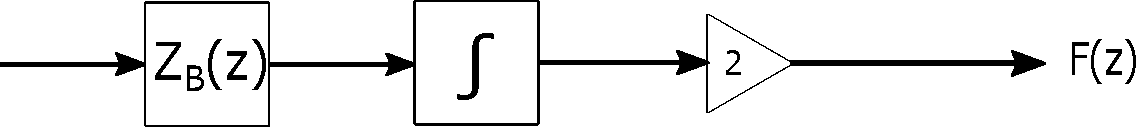
\includegraphics[width=0.9\linewidth]{H_B.pdf}
		\caption{}
		\label{fig:hb}
	\end{subfigure}
	\caption{Schematics of the filter components. See Section 3 for the sampling frequency.}
\end{figure}

The resulting $H_{EB}$ has been plotted as a function of the frequency in Fig. \ref{fig:q2}. We simulated the E\textsubscript{2} string of an acoustic guitar, taking as scale length the nominal value of $25.4''$ of a Martin D-28 and with $\mu = \SI{5.78}{\gram\per\meter}$. The plucking happens at 1/5 of the length of the string. At $\sim126$ Hz and $\sim270$ Hz we can see the modes of the bridge impedance. Moreover, we can see resonances at the fundamental (82 Hz) and its multiples. Notice how the resonance at the fifth harmonic appears less pronounced than the others, as expected.


\begin{figure}[h]
	\centering
	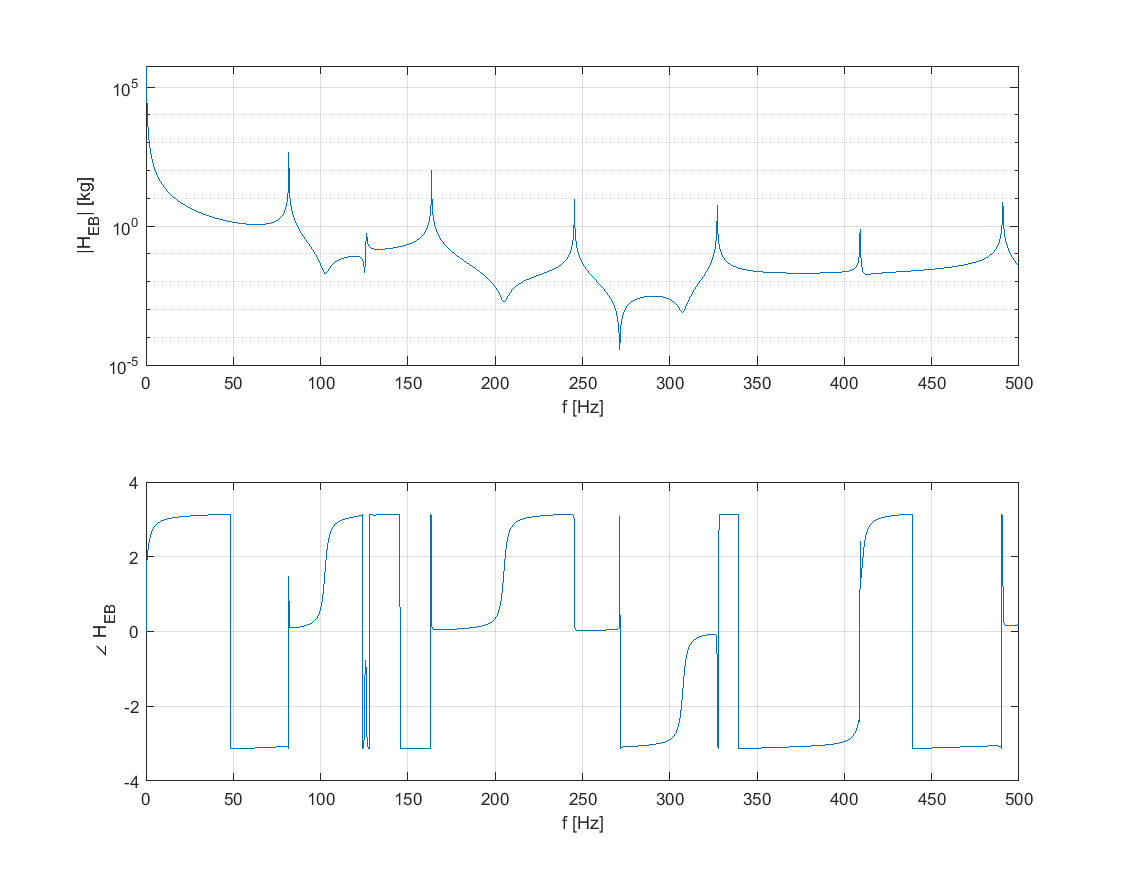
\includegraphics[width=0.75\linewidth]{heb.png}
	\caption{Magnitude and phase of $H_{EB}(\mathrm{j}\omega)$.}
	\label{fig:q2}
\end{figure}



\section{Making a sound: the time domain response}

We now turn to investigating the response of our model to a pluck with maximum displacement $d = \SI{3}{\milli\meter}$. We follow here \cite{smith92} to obtain a suitable If $\beta L$ is the distance from the bridge to the plucking point, the initial configuration of the string will be:
$$ 
y(x, 0) = \left\{
	\begin{array}{lr}
		\frac{d}{\beta L}x & x \in [0, \beta L] \\[4pt]
		d \bigl[ 1 - \frac{x}{(1 - \beta) L} \bigr] & x \in [\beta L, L]
	\end{array}
\right.
$$
We can recover the initial acceleration noting that, thanks to the wave equation, it is proportional to the curvature of the string $\frac{\partial^2 y}{\partial x^2}$. The result is a Dirac delta centered in the plucking point:
$$
\ddot y(x, 0) = c^2 \biggl( \frac{d}{\beta L} + \frac{d}{(1 - \beta) L} \biggr) \delta(x - \beta L).
$$
Now, when implementing a digital waveguide we need to sample both the time and the spatial variable. The sampling interval in time and the sampling interval in space must satisfy $X = cT$, where $c$ is the wave velocity in the string. Furthermore, the input needs to be bandlimited in the spatial frequency. If we use an ideal lowpass for antialiasing and convolve it with the impulse, we get $\ddot y (x, 0) \propto \mathrm{sinc}\left( \frac{x-\beta L}{X} \right)$. If $\beta L$ is an integer multiple of $X$, this becomes a discrete impulse, which allows us to lump the excitation on a single point of the waveguide and thus to commute the components of the filters like we saw in the previous section.

Fig. \ref{fig:dleng} shows the time history of the force on the bridge when using the input described above.


\begin{figure}[h]
	\centering
	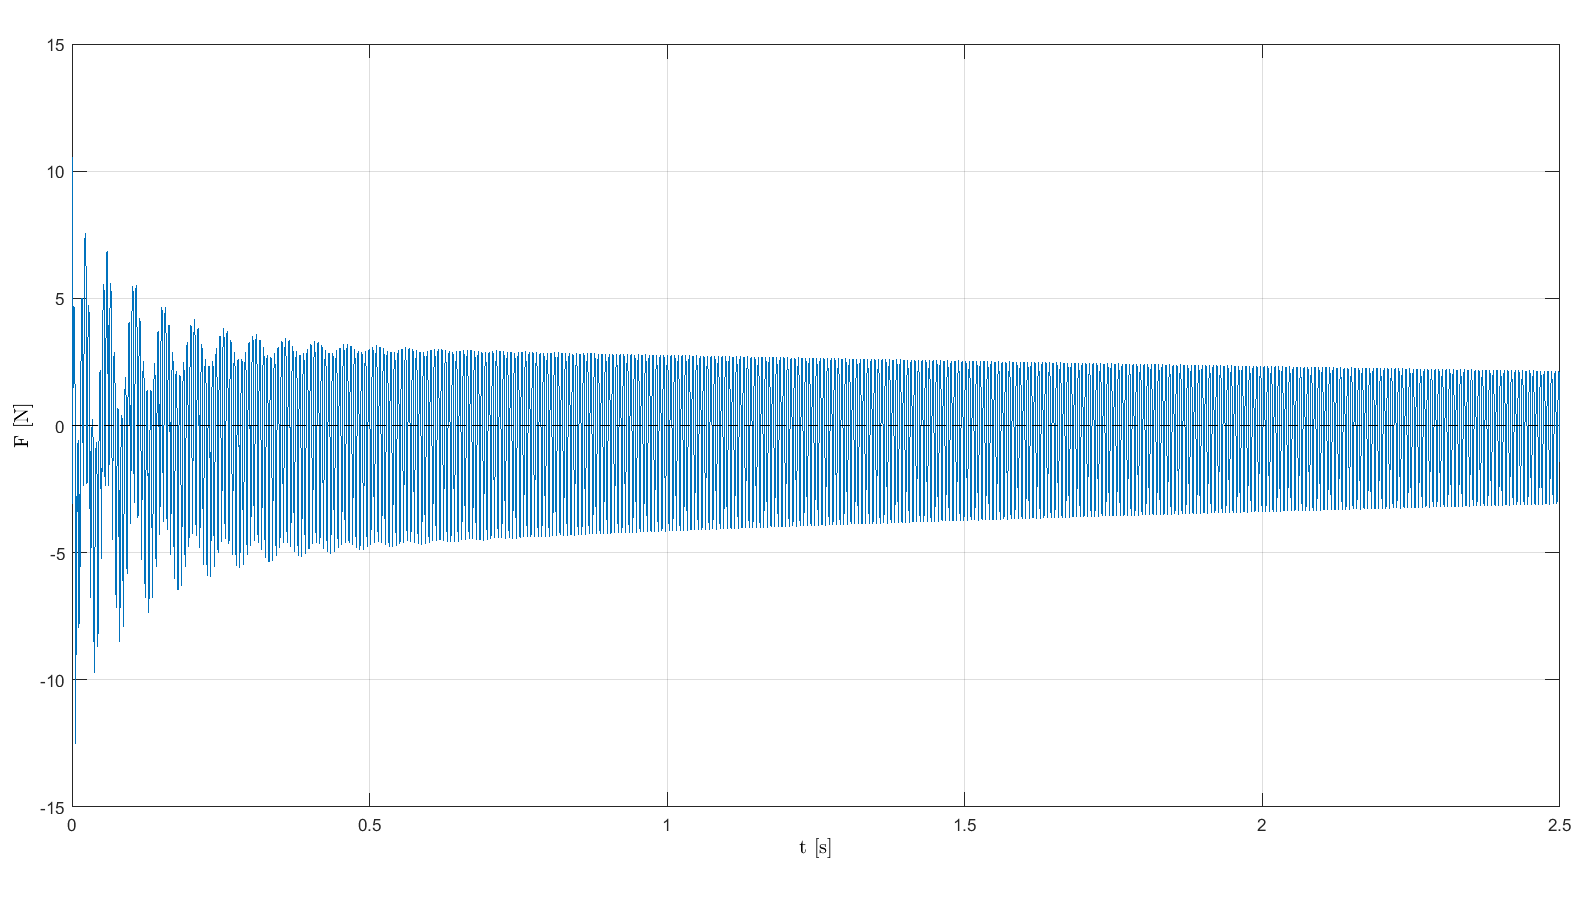
\includegraphics[width=0.75\linewidth]{time.png}
	\caption{Time history of the force on the bridge.}
	\label{fig:dleng}
\end{figure}




\end{document}